\begin{pastexam}[label={px:df3-113-ds-04}]{地方三等資訊處理 113 年 第四題}
（申論；25 分）

關於紅黑樹（Red Black Tree）與(2,4)-樹((2,4)-Tree)：
\begin{enumerate}[leftmargin=2.6em, labelsep=0.4em]
\item[㈠] 請分別說明紅黑樹與(2,4)-樹的定義。（10 分）
\item[㈡] 考慮下面的紅黑樹（實線節點代表黑色節點，虛線節點代表紅色節點），代表節點的字元符號可視為鍵值，
請說明如何將此紅黑樹轉換為一個(2,4)-樹，並將其結果畫出。此外，請申論轉換的(2,4)-樹是否唯一。（10 分）
\begin{center}
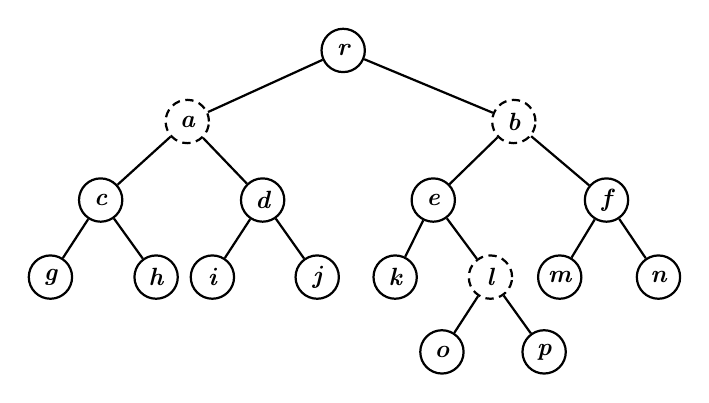
\begin{tikzpicture}[x=1.1cm,y=0.95cm,bn/.style={circle,draw,thick,inner sep=0pt,minimum size=5.5mm,font=\small\bfseries\itshape},
  rn/.style={bn,densely dashed}]
\node[bn] (r) at (3.38,0) {r};
\node[rn] (a) at (1.58,-0.95) {a};
\node[rn] (b) at (5.35,-0.95) {b};
\node[bn] (c) at (0.58,-2.0) {c};
\node[bn] (d) at (2.45,-2.0) {d};
\node[bn] (e) at (4.42,-2.0) {e};
\node[bn] (f) at (6.42,-2.0) {f};
\node[bn] (g) at (0,-3.03) {g};
\node[bn] (h) at (1.22,-3.03) {h};
\node[bn] (i) at (1.87,-3.03) {i};
\node[bn] (j) at (3.08,-3.03) {j};
\node[bn] (k) at (3.98,-3.03) {k};
\node[rn] (l) at (5.08,-3.03) {l};
\node[bn] (m) at (5.88,-3.03) {m};
\node[bn] (n) at (7.02,-3.03) {n};
\node[bn] (o) at (4.52,-4.03) {o};
\node[bn] (p) at (5.7,-4.03) {p};
\draw[thick] (r)--(a) (r)--(b) (a)--(c) (a)--(d) (b)--(e) (b)--(f) (c)--(g) (c)--(h) (d)--(i) (d)--(j)
  (e)--(k) (e)--(l) (f)--(m) (f)--(n) (l)--(o) (l)--(p);
\end{tikzpicture}
\end{center}
\item[㈢] 請說明為何一個有 $n$ 個節點（鍵值）的紅黑樹其高度是 O($\log n$)。（5 分）
\end{enumerate}
\end{pastexam}

\begin{pastsoln}
圖中的字母只是節點的名字，並沒有照字母順序排（例如 $a$ 在 $r$ 的左邊、$c$ 又在 $a$ 的左邊）。 以下把鍵值的
大小順序當成樹的中序：$g, c, h, a, i, d, j, r, k, e, o, l, p, b, m, f, n$ 由小到大。 先檢查這確實是合法的紅黑樹：
紅色節點是 $a$、$b$、$l$，它們的子節點都是黑色；從根到任何一個 NIL 的路徑都經過 $3$ 個黑色節點（例如
$r, c, g$；$r, e, o$），黑高度一致。

\textbf{㈠ 定義}。

\textbf{紅黑樹}（資結書第~10.3~節）是一棵二元搜尋樹，每個節點多存一個顏色，並滿足：
\begin{enumerate}[label=(\arabic*)]
\item 每個節點是紅色或黑色；
\item 根是黑色；
\item 每個葉節點（NIL，空的外部節點）是黑色；
\item 紅色節點的兩個子節點都是黑色（不會有兩個紅色節點相連）；
\item 對每個節點，從它到其子孫中任一個 NIL 的所有路徑上，黑色節點的個數都相同（這個數稱為黑高度）。
\end{enumerate}

\textbf{(2,4)-樹}（又叫 2-3-4 樹，資結書第~11.1.5~節）是一棵多路搜尋樹，滿足：
\begin{enumerate}[label=(\arabic*)]
\item \textbf{大小}：每個內部節點有 $2$、$3$ 或 $4$ 個子節點，分別存 $1$、$2$、$3$ 個鍵值；有 $d$ 個子節點的
節點存 $d - 1$ 個由小到大排列的鍵值 $k_1 < \cdots < k_{d-1}$，第 $i$ 棵子樹的鍵值都介於 $k_{i-1}$ 和 $k_i$ 之間。
\item \textbf{深度}：所有葉節點（外部節點）都在同一層。
\end{enumerate}

\textbf{㈡ 轉換}（資結書第~10.4~節）：把每個紅色節點「併入」它的黑色父節點。 由性質 (4)，紅色節點的父節點
一定是黑色，所以每個黑色節點連同它的紅色子節點（$0$、$1$ 或 $2$ 個）合成一個 (2,4)-樹的節點，有 $1$ 到 $3$
個鍵值，鍵值照中序排；合併後節點的子節點，是這一群節點底下的那些黑色子節點。 逐一處理：
\begin{itemize}
\item $r$（黑）有兩個紅子 $a$、$b$：合成 $[\,a\;r\;b\,]$。 它的子節點是 $a$ 的子 $c, d$ 和 $b$ 的子 $e, f$，共 $4$ 個。
\item $c$、$d$、$f$（黑）沒有紅子：各自成為 $[\,c\,]$、$[\,d\,]$、$[\,f\,]$，各有 $2$ 個子節點。
\item $e$（黑）有一個紅子 $l$：合成 $[\,e\;l\,]$（中序 $e$ 在 $l$ 前），子節點是 $k$ 和 $l$ 的子 $o, p$，共 $3$ 個。
\item $g, h, i, j, k, o, p, m, n$ 都是黑色、子節點都是 NIL，各成為只有一個鍵值的葉層節點。
\end{itemize}
結果（每個方框是一個 (2,4)-樹的節點，最下層節點的子節點都是外部節點，省略不畫）：
\begin{center}
\begin{tikzpicture}[x=1cm,y=1cm,k/.style={draw,rectangle,inner sep=3pt,minimum height=6mm,font=\small\itshape}]
\node[k] (R) at (0,0) {a\;\,$|$\;\,r\;\,$|$\;\,b};
\node[k] (C) at (-4.2,-1.4) {c};
\node[k] (D) at (-1.9,-1.4) {d};
\node[k] (E) at (1.4,-1.4) {e\;\,$|$\;\,l};
\node[k] (F) at (4.2,-1.4) {f};
\node[k] (G) at (-4.9,-2.8) {g};
\node[k] (H) at (-3.5,-2.8) {h};
\node[k] (I) at (-2.6,-2.8) {i};
\node[k] (J) at (-1.2,-2.8) {j};
\node[k] (K) at (0.3,-2.8) {k};
\node[k] (O) at (1.4,-2.8) {o};
\node[k] (P) at (2.5,-2.8) {p};
\node[k] (M) at (3.5,-2.8) {m};
\node[k] (N) at (4.9,-2.8) {n};
\draw ($(R.south west)!0.08!(R.south east)$) -- (C.north);
\draw ($(R.south west)!0.36!(R.south east)$) -- (D.north);
\draw ($(R.south west)!0.64!(R.south east)$) -- (E.north);
\draw ($(R.south west)!0.92!(R.south east)$) -- (F.north);
\draw (C.south) -- (G.north); \draw (C.south) -- (H.north);
\draw (D.south) -- (I.north); \draw (D.south) -- (J.north);
\draw ($(E.south west)!0.1!(E.south east)$) -- (K.north);
\draw (E.south) -- (O.north);
\draw ($(E.south west)!0.9!(E.south east)$) -- (P.north);
\draw (F.south) -- (M.north); \draw (F.south) -- (N.north);
\end{tikzpicture}
\end{center}
這是合法的 (2,4)-樹：根有 $4$ 個子節點、$[\,e\;l\,]$ 有 $3$ 個、其他內部節點 $2$ 個；一個節點的深度等於紅黑樹
裡從根到它的路徑上黑色節點的個數（減 $1$），由性質 (5) 所有葉層節點都在第 $3$ 層。

\textbf{唯一嗎？} 從\textbf{一棵給定的紅黑樹}轉換，結果是唯一的：每個紅色節點只有一個父節點，該併到哪個節點
沒有選擇，合併後的鍵值順序也由中序決定。 但反過來不唯一：同一棵 (2,4)-樹可以對應好幾棵紅黑樹。 $2$ 個鍵值的
節點有兩種畫法，例如 $[\,e\;l\,]$ 可以是「$e$ 黑、右子 $l$ 紅」（本題），也可以是「$l$ 黑、左子 $e$ 紅」，此時
$k, o$ 掛在 $e$ 底下、$p$ 掛在 $l$ 的右邊；$1$ 個鍵值和 $3$ 個鍵值的節點則只有一種畫法（$3$ 個鍵值時中間的黑、
兩旁的紅）。 所以這棵 (2,4)-樹只有一個 $2$ 鍵值節點，對應 $2$ 棵紅黑樹；一般有 $t$ 個 $2$ 鍵值節點的 (2,4)-樹
對應 $2^t$ 棵紅黑樹。

\textbf{㈢ 高度是 $O(\log n)$}。 令 $b$ 為從根到任一 NIL 的路徑上黑色節點的個數（含根、不含 NIL）；由性質 (5)，
每條路徑都一樣。
\begin{itemize}
\item \textbf{黑色節點夠多}：照㈡的方法轉成 (2,4)-樹，這棵樹恰好有 $b$ 層節點，每個內部節點至少有 $2$ 個子節點，
所以第 $1, 2, \ldots, b$ 層至少有 $1, 2, \ldots, 2^{b-1}$ 個節點，每個節點至少一個鍵值，共
$n \ge 2^b - 1$ 個鍵值，即 $b \le \lg(n + 1)$。
\item \textbf{紅色節點不會太多}：最長的根到 NIL 路徑上有 $h$ 個節點（$h$ 是樹高）。 由性質 (4)，紅色節點的下一個
一定是黑色（或 NIL），根又是黑色，所以路徑上紅色節點不比黑色多，$h \le 2b$。
\end{itemize}
合起來 $h \le 2b \le 2\lg(n + 1) = O(\log n)$（資結書定理~10.4）。 以本題為例：$n = 17$，$b = 3$，最長路徑
$r \to b \to e \to l \to o$ 有 $5$ 個節點，$5 \le 2 \cdot 3 \le 2\lg 18 \approx 8.3$。 所以搜尋、插入、刪除的時間
都是 $O(\log n)$。
\end{pastsoln}
